\documentclass[11pt,a4paper]{article}
\usepackage[T1]{fontenc}
\usepackage[utf8]{inputenc}
\usepackage{lmodern,microtype}
\usepackage[margin=25mm,headheight=15pt]{geometry}
\usepackage{amsmath,amssymb,amsthm,mathtools}
\usepackage{graphicx,booktabs,array,multirow}
\usepackage{caption,subcaption,float}
\usepackage{enumitem,xcolor}
\usepackage{fancyhdr}
\usepackage{hyperref}
\hypersetup{colorlinks=true,linkcolor=blue!55!black,citecolor=blue!55!black,urlcolor=blue!55!black,pdftitle={The Paradox of Absolute Luck: Can Probability Favor Everyone?},pdfauthor={Anonymous expository manuscript draft}}
\definecolor{ink}{HTML}{172B43}
\definecolor{muted}{HTML}{54718B}
\definecolor{line}{HTML}{D5E0E9}
\usepackage{tcolorbox}
\tcbuselibrary{breakable}
\pagestyle{fancy}
\fancyhf{}
\fancyhead[L]{\small\textcolor{muted}{ABSOLUTE LUCK / MATHEMATICAL EXPOSITION}}
\fancyhead[R]{\small\textcolor{muted}{PHASE 6 -- 7 NOV 2026}}
\fancyfoot[C]{\thepage}
\renewcommand{\headrulewidth}{0.3pt}
\captionsetup{font=small,labelfont=bf,justification=raggedright,singlelinecheck=false}
\setlength{\parindent}{0pt}
\setlength{\parskip}{6pt}
\setlist[itemize]{noitemsep,topsep=4pt,leftmargin=15pt}
\newtheorem{proposition}{Proposition}
\newtheorem{corollary}[proposition]{Corollary}
\newtheorem{remark}[proposition]{Remark}
\newtheorem{example}[proposition]{Example}
\newcommand{\PP}{\mathbb{P}}
\newcommand{\EE}{\mathbb{E}}
\newcommand{\Cov}{\operatorname{Cov}}
\newcommand{\Var}{\operatorname{Var}}
\newcommand{\TV}{\operatorname{TV}}
\begin{document}

\begin{center}
{\large\textcolor{muted}{EXPOSITORY MATHEMATICS / SYNTHETIC COMPUTATIONAL STUDY}}\\[7pt]
{\huge\bfseries\textcolor{ink}{The Paradox of Absolute Luck}}\\[5pt]
{\Large\textcolor{ink}{Can Probability Favor Everyone?}}\\[8pt]
{\large Competing guarantees, joint success, and the assumptions behind near-certainty}\\[10pt]
{\normalsize Anonymous manuscript draft \quad|\quad 7 November 2026}\\[4pt]
\end{center}
\begin{tcolorbox}[colback=blue!3,colframe=line,boxrule=0.5pt,arc=2pt,breakable]
\textbf{Research classification.} A rigorous \emph{expository} investigation combining established probability theory with exact thought experiments and reproducible synthetic simulations. It does not present a newly discovered theorem, measured comic outcomes, or an empirically validated mechanism of ``luck.'' The companion narrative essay is reserved for Phase 7.
\end{tcolorbox}
\begin{abstract}
A fictional ability that makes a favorable event nearly certain poses an apparently paradoxical question: can two opponents both be overwhelmingly likely to win, and can hundreds of individually reliable events jointly fail with certainty? We formalize these questions as constraints on probability models. Mutually exclusive victories cannot each have probability $0.99$ in one contest, yet equal $0.99$ performance against a common baseline does not identify the head-to-head result. Sharp Fr\'echet--Boole bounds show that $200$ exchangeable Bernoulli outcomes can each succeed with probability $0.995$ even when their conjunction has probability zero. That law, however, cannot be extended exchangeably to $201$ variables, whereas an infinitely exchangeable sequence satisfies a qualitatively different lower bound. We also construct two three-variable laws with identical one- and two-coordinate distributions but different triple-success probabilities, and a fixed dependence mechanism under which a reliability-allocation ranking reverses relative to independence. Exact proofs are accompanied by a preserved seeded Monte Carlo study with $120{,}000$ trials per main scenario, confidence-interval diagnostics, and model-discrimination experiments. The contribution is an explicitly scoped mathematical synthesis: no fictional probability rule or mathematical novelty is inferred from the examples.
\end{abstract}
\textbf{Keywords:} Fr\'echet bounds; joint probability; exchangeability; probabilistic choice; identifiability; Bernoulli dependence; Monte Carlo; reliability allocation.

\section{Introduction and scope}

The narrative premise comes from \emph{Hardcore Leveling Warrior}, a fictional series by Sehoon Kim \cite{webtoon}. The work motivates a thought experiment about extreme favorable outcomes, not an observational data source. We make no claim to have authenticated numerical Lucky Coin activation rates, counted panels as experiments, or inferred the actual probability law of any fictional ability. All numerical parameters below are selected mathematical examples.

The apparent ``luck paradox'' is a model-specification problem. Probability statements only become comparable once the experiment, relevant event, and context are fixed. In a single-winner duel, two distinct victory events are disjoint; in a coin batch, multiple successes may coexist but need not be independent. The same adjective, \emph{lucky}, can refer to a conditional relative preference, a fixed marginal probability, a higher-order dependence structure, or a resource-dependent probability transformation.

We organize the investigation around five established mathematical observations illustrated by concrete constructions: (i) coherence constraints in a zero-sum contest; (ii) extremal intersections with fixed marginals; (iii) limitations of lower-order data; (iv) finite versus infinite exchangeability; and (v) dependence-sensitive allocation. The probabilistic tools and related research are classical or already studied, including choice models \cite{bradley,luce}, optimal joint-event bounds \cite{hoppe}, exchangeability \cite{kirsch,konstantopoulos}, and reliability allocation \cite{shaked}. Our aim is a self-contained, testable explanation rather than a novel-theorem claim.

\section{General formalism: the missing context}

Let $c$ index a fully specified experimental context and $(\Omega_c,\mathcal F_c,\PP_c)$ its probability space. For an event $E_i(c)\in\mathcal F_c$, write $p_i(c)=\PP_c(E_i(c))$. Statements such as $p_i(c_1)=0.99$ and $p_j(c_2)=0.99$ need not constrain a common event space when $c_1\ne c_2$. By contrast, if mutually exclusive $E_1(c)$ and $E_2(c)$ belong to the same experiment, their probabilities must sum to at most one.

The phrase ``one coin succeeds with $99.5\%$ probability'' could mean that a coin activated alone has success probability $0.995$, or that it retains this probability within an $n$-coin batch. Those are different assumptions. We distinguish (a) \textbf{isolated context}, (b) \textbf{batch context}, and (c) \textbf{observation protocol} throughout.

\section{Paradox I: two supposedly certain winners}

\begin{proposition}[The collision coherence constraint]\label{prop:collision}
In a contest with at most one winner, events $A$ and $B$ denoting victory by two distinct entrants obey $\PP(A)+\PP(B)\leq1$. In particular, $\PP(A)=\PP(B)=0.99$ is impossible in the same contest and the same probability space.
\end{proposition}
\begin{proof}
The events are disjoint, so $\PP(A\cup B)=\PP(A)+\PP(B)\leq\PP(\Omega)=1$.
\end{proof}

The proposition does \emph{not} say two contestants cannot each beat an ordinary opponent with probability $0.99$ in different contests. Consider one possible resolution: assign positive stable weights $w_i$ and set
\begin{equation}\label{eq:luce}
\PP(i\text{ wins}\mid S)=\frac{w_i}{\sum_{j\in S}w_j},\qquad i\in S.
\end{equation}
For $w_A=w_B=99$ and $w_N=1$, both A and B beat ordinary N with probability $0.99$, but A defeats B with probability $1/2$. Equation \eqref{eq:luce} is a weighted choice assumption closely associated with Bradley--Terry/Luce models, not a consequence of probability axioms \cite{bradley,luce}. Its odds $\PP(i\mid S)/\PP(j\mid S)=w_i/w_j$ do not depend on other alternatives in $S$.

\begin{proposition}[Equal baseline performance does not identify the duel]\label{prop:ranking}
There exists a single coherent probability law in which $\PP(A>N)=\PP(B>N)=0.99$ but $\PP(A>B)=0.90$.
\end{proposition}
\begin{proof}
Draw one complete ranking from $A>B>N$, $B>A>N$, and $N>A>B$ with probabilities $0.89$, $0.10$, and $0.01$, respectively. The higher-ranked player wins every subcontest. Both A and B defeat N unless the third ranking occurs, so each wins against N with probability $0.99$. A defeats B in the first and third rankings, with total probability $0.89+0.01=0.90$. Every matchup derives from the same distribution on complete rankings.
\end{proof}

Thus two matching favorable statistics do not define a universal, opponent-independent ``luck percentage.'' A $50$--$50$ duel follows from stable equal weights or exchange symmetry, not from equality of baseline win rates alone.

\begin{figure}[H]
\centering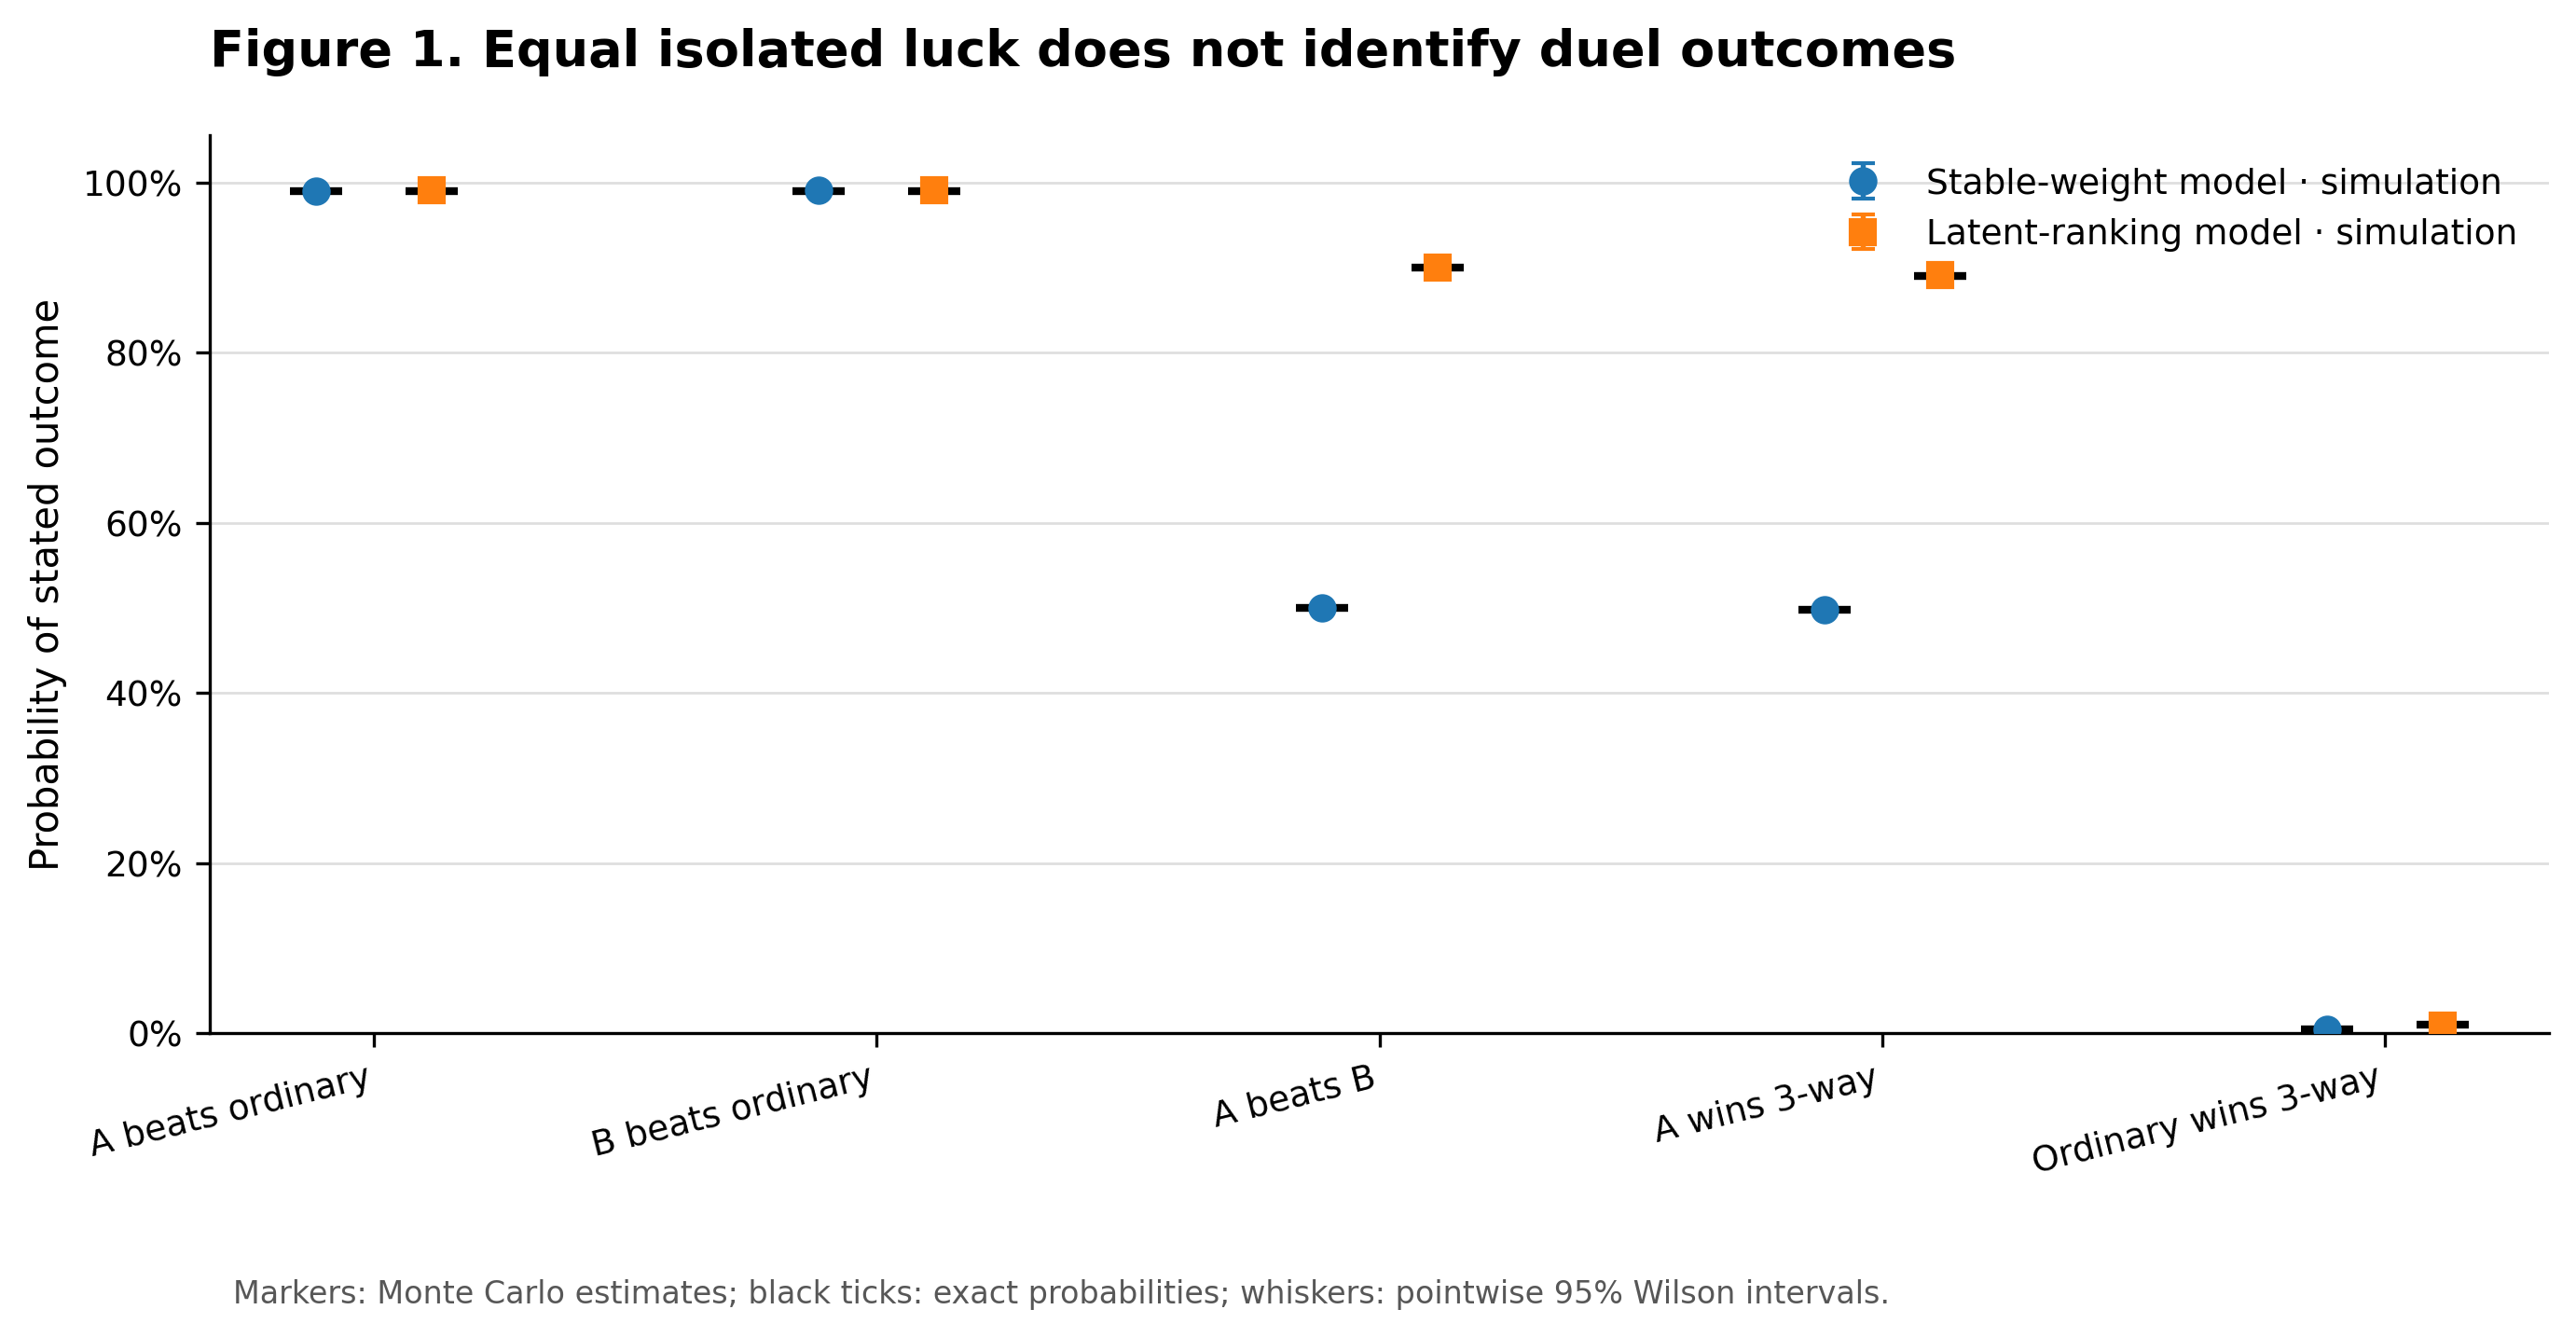
\includegraphics[width=.94\linewidth]{figures/fig01_collision.png}
\caption{\textbf{Context-sensitive competition.} Theory and seeded simulation for a stable weighted-choice law and a coherent latent-ranking countermodel. All rates are synthetic.}\label{fig:collision}
\end{figure}

\section{Paradox II: from near-certainty to joint failure}

For Bernoulli success indicators $X_1,\ldots,X_n$, let $E_i=\{X_i=1\}$ and $J_n=\PP(\cap_i E_i)$.

\begin{proposition}[Sharp intersection bounds]\label{prop:frechet}
For any events $E_i$ with $\PP(E_i)=p_i$,
\begin{equation}\label{eq:bounds}
\max\left\{0,\sum_{i=1}^n p_i-(n-1)\right\}\leq J_n\leq\min_i p_i.
\end{equation}
The endpoints can be attained over suitable joint distributions with the stated marginals.
\end{proposition}
\begin{proof}
Apply the union bound to failures: $1-J_n=\PP(\cup_i E_i^c)\leq\sum_i(1-p_i)$; nonnegativity gives the lower bound. Since $\cap_iE_i\subseteq E_j$ for each $j$, $J_n\leq p_j$. Sharpness follows by arranging failure sets disjointly where their total measure is at most one, or to cover the full unit interval when their total measure is at least one; nesting success sets attains the upper endpoint. These are classical Fr\'echet--Boole bounds \cite{hoppe}.
\end{proof}

For three simultaneous coins each having marginal $0.995$, Equation \eqref{eq:bounds} forces $J_3\in[0.985,0.995]$. A claim that $J_3=0.60$ while all these \emph{same-context} marginals remain $0.995$ is inconsistent. If instead the batch marginals $p_i$ are allowed to change, then $J_3=0.60$ implies $\sum_i p_i\leq2.60$ and thus $\sum_i(0.995-p_i)\geq0.385$.

\begin{example}[Two hundred extraordinarily reliable coins]\label{ex:200}
Choose uniformly an index $I\in\{1,\ldots,200\}$ and let precisely coin $I$ fail. Each coin succeeds with probability $199/200=0.995$, but $J_{200}=0$, because at least one failure occurs in every outcome. This is a finite exchangeable distribution: its law is invariant under permutations of the 200 indices.
\end{example}

This does not assert that a batch of 200 independent coins must fail. Under independent Bernoulli$(0.995)$ sampling, $J_{200}=0.995^{200}\approx0.366958$. Under an alternative shared-latent model, let $\Theta\sim\mathrm{Beta}(199,1)$ and draw conditionally independent Bernoulli$(\Theta)$ outcomes; then $\EE\Theta=0.995$ and $J_{200}=\EE[\Theta^{200}]=199/399\approx0.498747$.

\begin{table}[H]
\centering\small
\caption{Same individual success probability, different 200-fold success. Simulations use independent trials; coins within a trial may be dependent.}\label{tab:200}
\begin{tabular}{@{}p{.42\linewidth}rr@{}}\toprule
Dependence model & Exact $J_{200}$ & Monte Carlo $\widehat J_{200}$ \\\midrule
Exactly one failure & $0.000\%$ & $0.000\%$ \\
Independent Bernoulli & $36.696\%$ & $36.568\%$ \\
Shared Beta parameter & $49.875\%$ & $49.753\%$ \\\bottomrule\end{tabular}
\end{table}

\begin{figure}[H]
\centering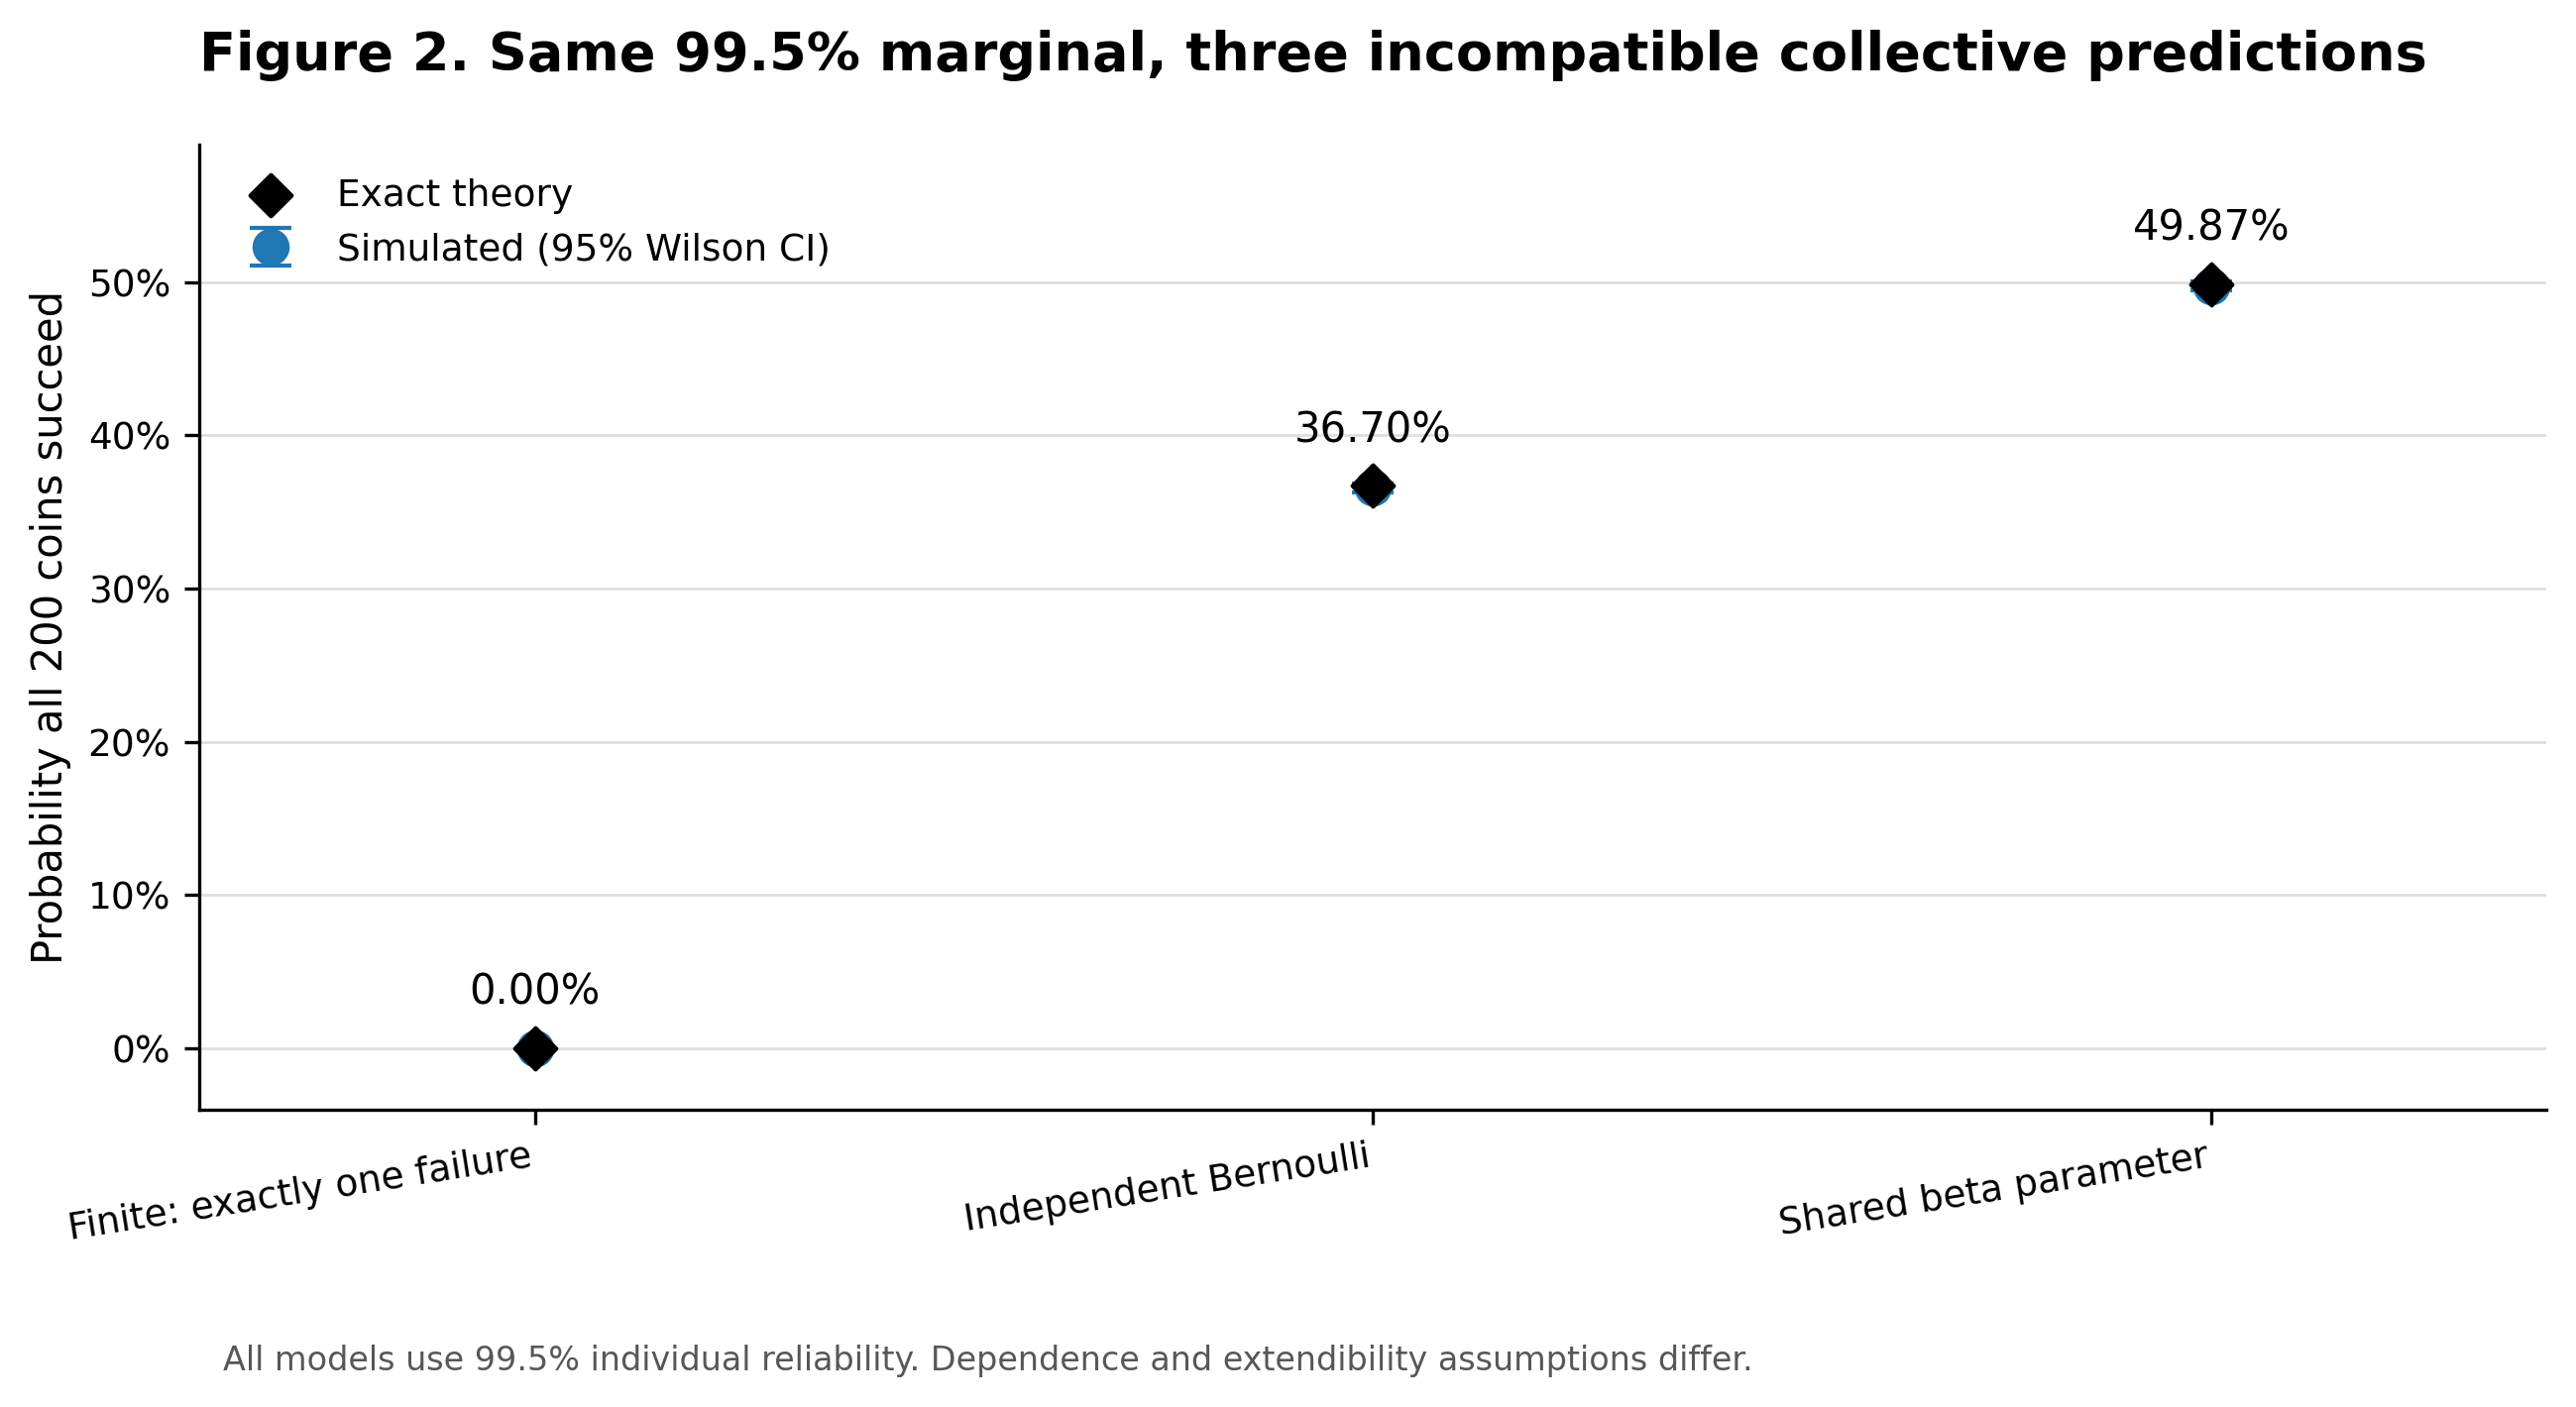
\includegraphics[width=.90\linewidth]{figures/fig02_joint_200_coins.png}
\caption{\textbf{The 200-coin contrast.} Theoretical joint-success probabilities and seeded Monte Carlo estimates under three stipulated laws, all with identical one-coin marginals of $0.995$.}\label{fig:200}
\end{figure}

\subsection{Why 200 valid coins may not admit a 201st symmetric coin}

\begin{proposition}[Failure of exchangeable extension]\label{prop:extension}
The law in Example \ref{ex:200} cannot be the 200-coordinate marginal of a 201-coordinate \emph{exchangeable} Bernoulli law. Its minimum total-variation distance from any such marginal is exactly $1/201$.
\end{proposition}
\begin{proof}
The original law has $\PP(X_i=1)=199/200$ and $\PP(X_i=X_j=1)=198/200$, hence covariance $-1/40000$ and correlation $\rho=-1/199$. For any $m$ exchangeable, nondegenerate Bernoulli variables, $0\leq\Var(\sum_iX_i)=m\Var(X_1)[1+(m-1)\rho]$, requiring $\rho\geq-1/(m-1)$. A 201-exchangeable extension would retain the original pair law and violate $\rho\geq-1/200$.

For sharp total variation, let $T$ denote the event that the first 200 coins contain exactly one failure. Condition on the number $R$ of failures among 201 exchangeable coins. The probability of $T$ is $200/201$ if $R=1$, $2/201$ if $R=2$, and zero otherwise; therefore it never exceeds $200/201$. The original law has $\PP(T)=1$, so its total variation from any candidate 200-marginal is at least $1/201$. If there is exactly one uniformly positioned failure among all 201 coins, the first-200 marginal equals $(200/201)$ times the desired 200-coin law plus $(1/201)$ times the all-success point mass. Its distance is exactly $1/201$.
\end{proof}

\begin{remark}[Finite versus infinite exchangeability]
De Finetti's theorem states that an \emph{infinitely} exchangeable Bernoulli sequence is a mixture of conditionally i.i.d. Bernoulli sequences \cite{kirsch}. Accordingly, for $n\ge2$ and $p=\EE\Theta$, Jensen's inequality yields
\begin{equation}\label{eq:jensen}
J_n=\EE[\Theta^n]\ge (\EE\Theta)^n=p^n,\qquad
\Cov(X_i,X_j)=\Var(\Theta)\ge0\quad(i\ne j).
\end{equation}
Neither conclusion applies to arbitrary \emph{finite} exchangeable laws. Extendibility itself is an established research topic \cite{konstantopoulos}.
\end{remark}

\section{Why one- and two-coin measurements may never identify the third}\label{sec:ident}

Consider exchangeable three-coin distributions that conditionally choose uniformly among all subsets with $K$ successes. Two choices for the mass function of $K$ are shown in Table \ref{tab:moment}.

\begin{table}[H]
\centering\small
\caption{Two exact exchangeable joint laws with identical full one- and two-coordinate distributions.}\label{tab:moment}
\begin{tabular}{@{}lcccc@{}}\toprule
 & $K=0$ & $K=1$ & $K=2$ & $K=3$ \\\midrule
Model L & $0.10$ & $0$ & $0.60$ & $0.30$ \\
Model H & $0$ & $0.30$ & $0.30$ & $0.40$ \\\bottomrule\end{tabular}
\end{table}

\begin{proposition}[Sharp higher-order ambiguity]\label{prop:ident}
If three exchangeable Bernoulli variables obey $\PP(X_i=1)=0.70$ and $\PP(X_i=X_j=1)=0.50$ for $i\ne j$, their triple-success probability $t=\PP(X_1=X_2=X_3=1)$ can be any value in the sharp interval $[0.30,0.40]$.
\end{proposition}
\begin{proof}
Write $q_k=\PP(K=k)$. Exchangeability gives $\EE K=3(0.70)=2.1$ and $\EE[K(K-1)]=6(0.50)=3$. Solving the normalization and moment equations with $q_3=t$ yields $q_0=0.4-t$, $q_1=-0.9+3t$, $q_2=1.5-3t$, $q_3=t$. Nonnegativity is equivalent to $0.3\le t\le0.4$. These endpoints are realized by Models L and H.
\end{proof}

Under the \emph{restricted observation protocol} that each independent trial reveals at most one coordinate or one pair, the complete distribution of observations is identical under Models L and H: for a pair, $\PP(11)=0.50$, $\PP(10)=\PP(01)=0.20$, $\PP(00)=0.10$. Thus no classifier can discriminate them better than $50\%$ expected accuracy with equal priors. This impossibility does not apply if observations from distinct pairs are linked to the \emph{same} triple realization; such records can encode higher-order information.

When complete triple outcomes are observed, let a prespecified classifier predict H if the empirical all-success rate is at least $0.35$. For $m$ independent triples and $k=\lceil0.35m\rceil$, its expected equal-prior accuracy is
\begin{equation}\label{eq:class}
1-\tfrac12\Big[\PP\{\mathrm{Bin}(m,0.30)\ge k\}+\PP\{\mathrm{Bin}(m,0.40)< k\}\Big].
\end{equation}
At $m=200$, Equation \eqref{eq:class} yields $93.17\%$ theoretical accuracy; at $m=500$, it yields $99.07\%$. The seeded replication gives $92.95\%$ and $99.25\%$, respectively, across 2,000 classifications at each sample size. The threshold is not claimed Bayes-optimal.

\begin{figure}[H]
\centering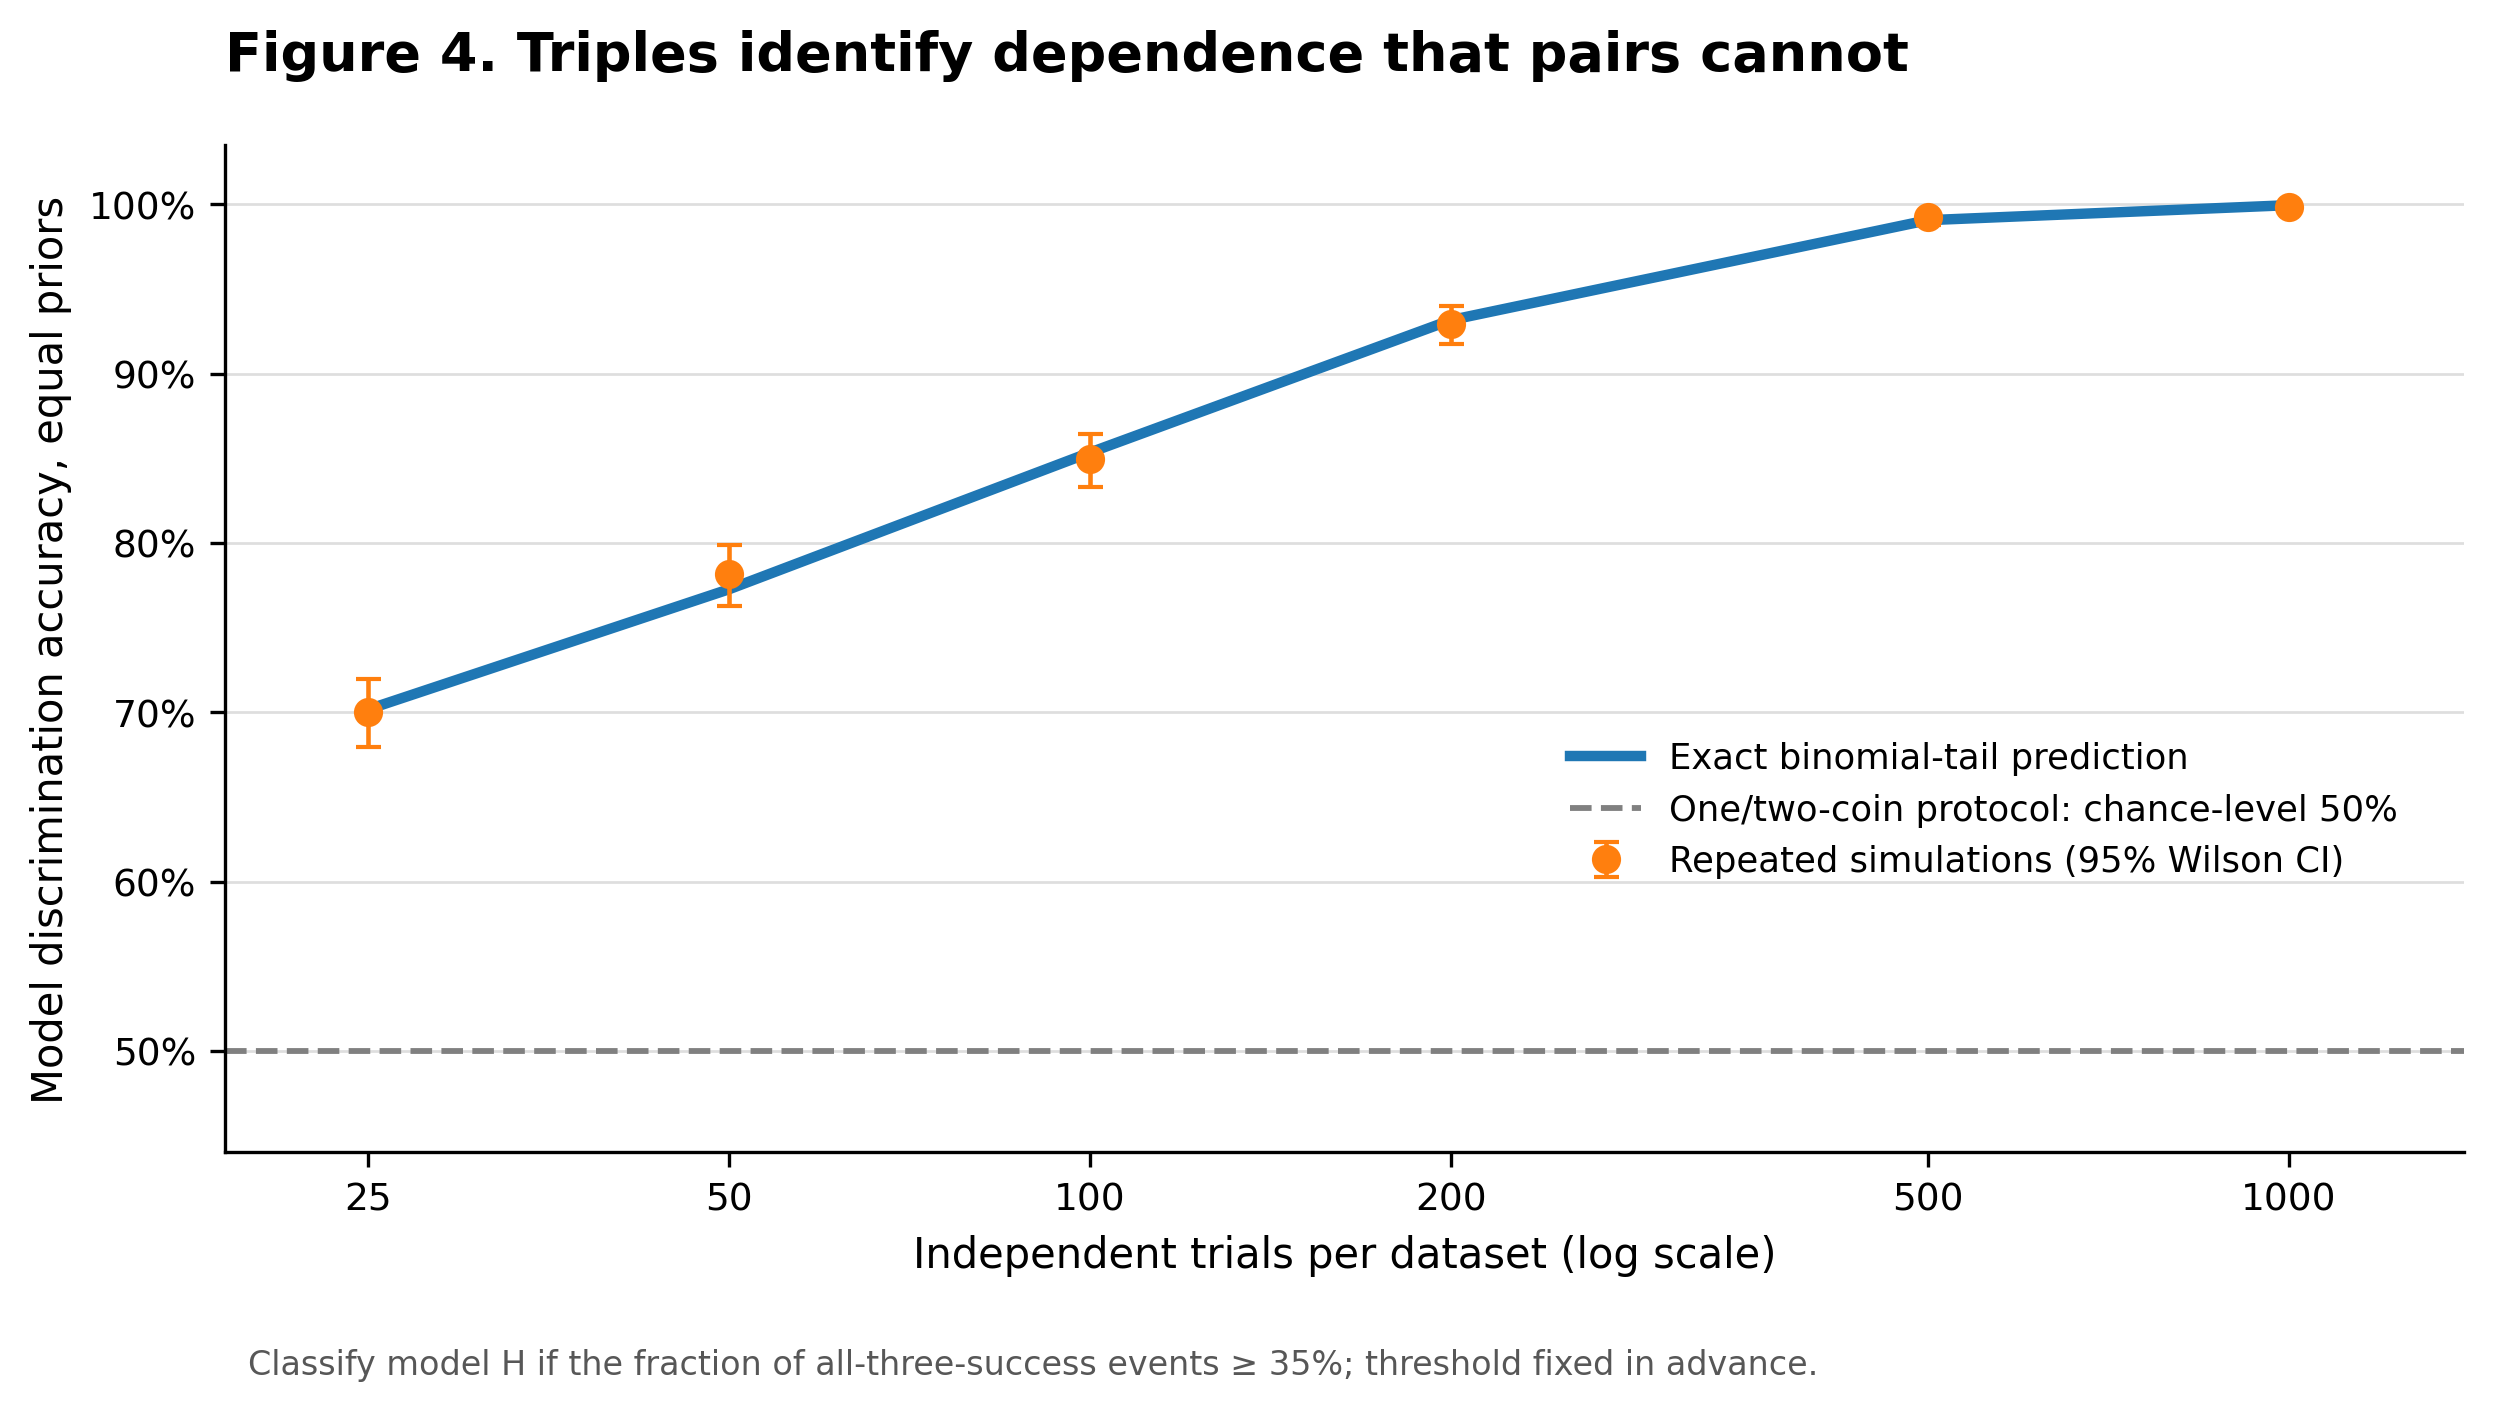
\includegraphics[width=.91\linewidth]{figures/fig04_identifiability.png}
\caption{\textbf{Identifying higher-order dependence.} Exact and simulated discrimination accuracy when full triple observations become available, contrasted with the unidentifiable one-/two-coordinate protocol.}\label{fig:ident}
\end{figure}

\section{A limited luck boost: objectives and dependence}

We now posit a completely hypothetical resource allocation: three coins have baseline success probability $1/2$, and nonnegative boosts $b_i$ obey $\sum_i b_i=B=0.495$, with $p_i=1/2+b_i$. This resource assumption is \emph{not} part of verified fictional canon.

Under independence, the all-success objective is $J_3=\prod_i p_i$. The arithmetic--geometric mean inequality yields the global maximum $J_3\le(1/2+B/3)^3=0.665^3=0.294079625$, reached at equal allocation. For a simple contrast, concentrated allocation $p=(0.995,0.5,0.5)$ gives $J_3=0.24875$.

Now hold a different but \emph{fixed} joint mechanism across both allocation strategies. Let $U\sim\mathrm{Unif}[0,1]$ and define
\begin{equation}\label{eq:copula}
X_1=\mathbf 1\{1-U\le p_1\},\quad X_2=\mathbf 1\{U\le p_2\},\quad X_3=\mathbf 1\{U\le p_3\}.
\end{equation}
All three marginal probabilities remain $p_i$, but
\begin{equation}\label{eq:fixed}
J_3=\max\{0,\min(p_2,p_3)-(1-p_1)\}.
\end{equation}
Equal allocation now gives $J_3=0.330$, while the same concentrated strategy gives $J_3=0.495$.

\begin{proposition}[Dependence reverses a policy ranking]\label{prop:reversal}
For the two allocations above, equal allocation gives larger all-success probability under independence, whereas concentrated allocation gives larger all-success probability under the single fixed coupling \eqref{eq:copula}.
\end{proposition}
\begin{proof}
Under independence, $0.665^3=0.294079625>0.995(0.5)^2=0.24875$. Under \eqref{eq:copula}, the all-success event is $1-p_1\le U\le\min(p_2,p_3)$; Equation \eqref{eq:fixed} gives $0.330<0.495$. The coupling rule has not changed between allocations.
\end{proof}

The proposition compares two policies only. It does \emph{not} establish that concentration globally maximizes \eqref{eq:fixed} across every feasible boost vector. Nor does it mean that independent and dependent regimes are empirically observed in the story. Comparable resource-allocation questions have a substantial reliability-theory history \cite{shaked}.

\begin{figure}[H]
\centering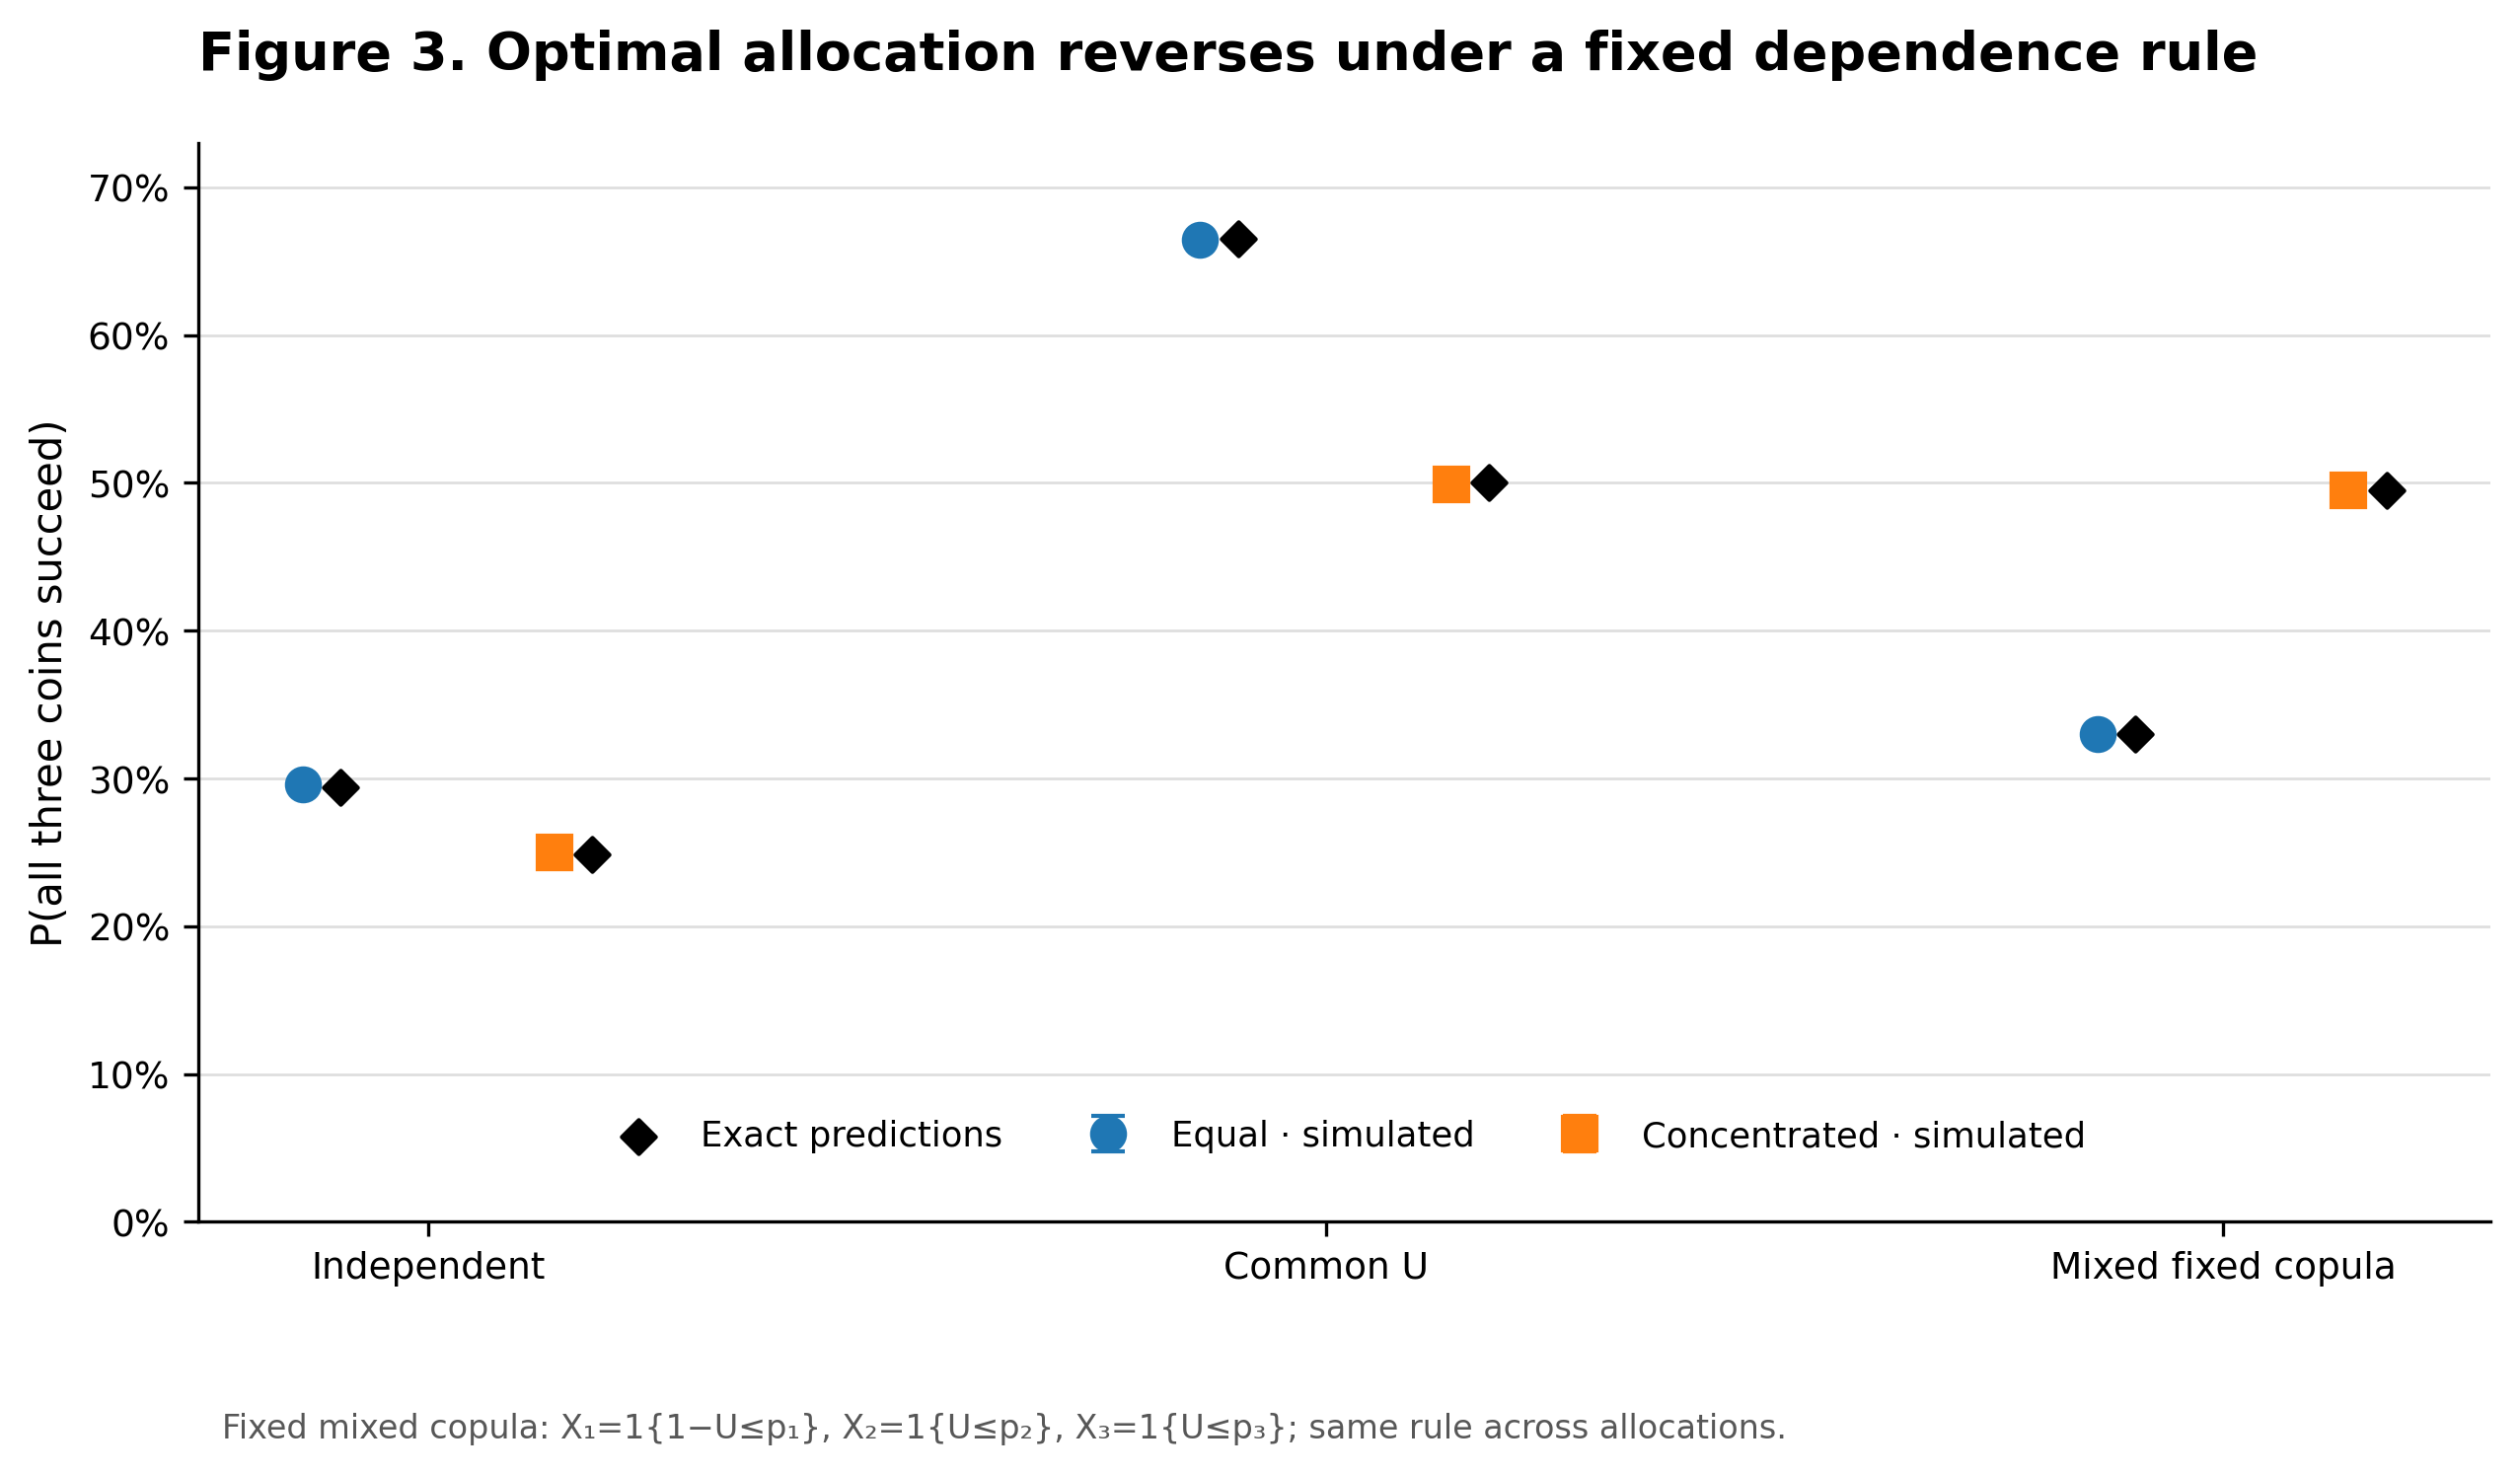
\includegraphics[width=.94\linewidth]{figures/fig03_allocation_dependence.png}
\caption{\textbf{Reliability allocation under three stipulated couplings.} Exact predictions and seeded estimates for equal and concentrated resource policies. Only the ranking of these two policies is compared.}\label{fig:allocation}
\end{figure}

\section{Reproducible numerical methodology}

The computations are carried forward from a frozen Phase 5 study plan, source code, and immutable input archive. For each main scenario, $120{,}000$ independent trials were generated using a NumPy PCG64 generator, base seed \texttt{20261107}, and scenario-specific derived streams. Independence is asserted \emph{between trials}, not between coin outcomes within a trial. Five figures were generated in both vector SVG and 300-DPI PNG formats; Figures \ref{fig:collision}--\ref{fig:allocation} reuse those archived outputs unchanged.

For an estimated Bernoulli probability $\hat p=k/n$, the pointwise approximate Wilson $95\%$ interval was used \cite{brown}:
\begin{equation}\label{eq:wilson}
\frac{\hat p+z^2/(2n)\pm z\sqrt{\hat p(1-\hat p)/n+z^2/(4n^2)}}{1+z^2/n},\quad z=\Phi^{-1}(0.975).
\end{equation}
The prespecified \emph{engineering} acceptance tolerance for each of 63 event-rate estimates was $|\hat p-p|\le 4.5\sqrt{p(1-p)/n}+0.00025$. This is not a simultaneous significance test. All 63 estimates passed this tolerance; eight of their pointwise Wilson intervals excluded the exact generating parameter, which is compatible with ordinary sampling variation and multiple interval comparisons.

For fixed-coupling policy comparisons, paired indicators used the same latent uniform draw in each trial. The exact concentrated-minus-equal all-success difference was $+0.165$; the Monte Carlo estimate was $+0.16485$, with a trial-level large-sample $95\%$ interval $[0.16098,0.16872]$. This interval is based on paired independent trials, not independent coins.

Separate identification studies generated 1,000 datasets from each candidate model at each sample size. A Wilson-coverage calibration used 600 independent datasets of 400 Bernoulli trials for each of five parameter values; observed pointwise coverage ranged from $93.67\%$ to $95.50\%$. These numbers are a finite simulation diagnostic, not a proof of universal coverage. Figure \ref{fig:convergence} shows sampling-error traces, which can fluctuate rather than improve monotonically with sample size.

\begin{figure}[H]
\centering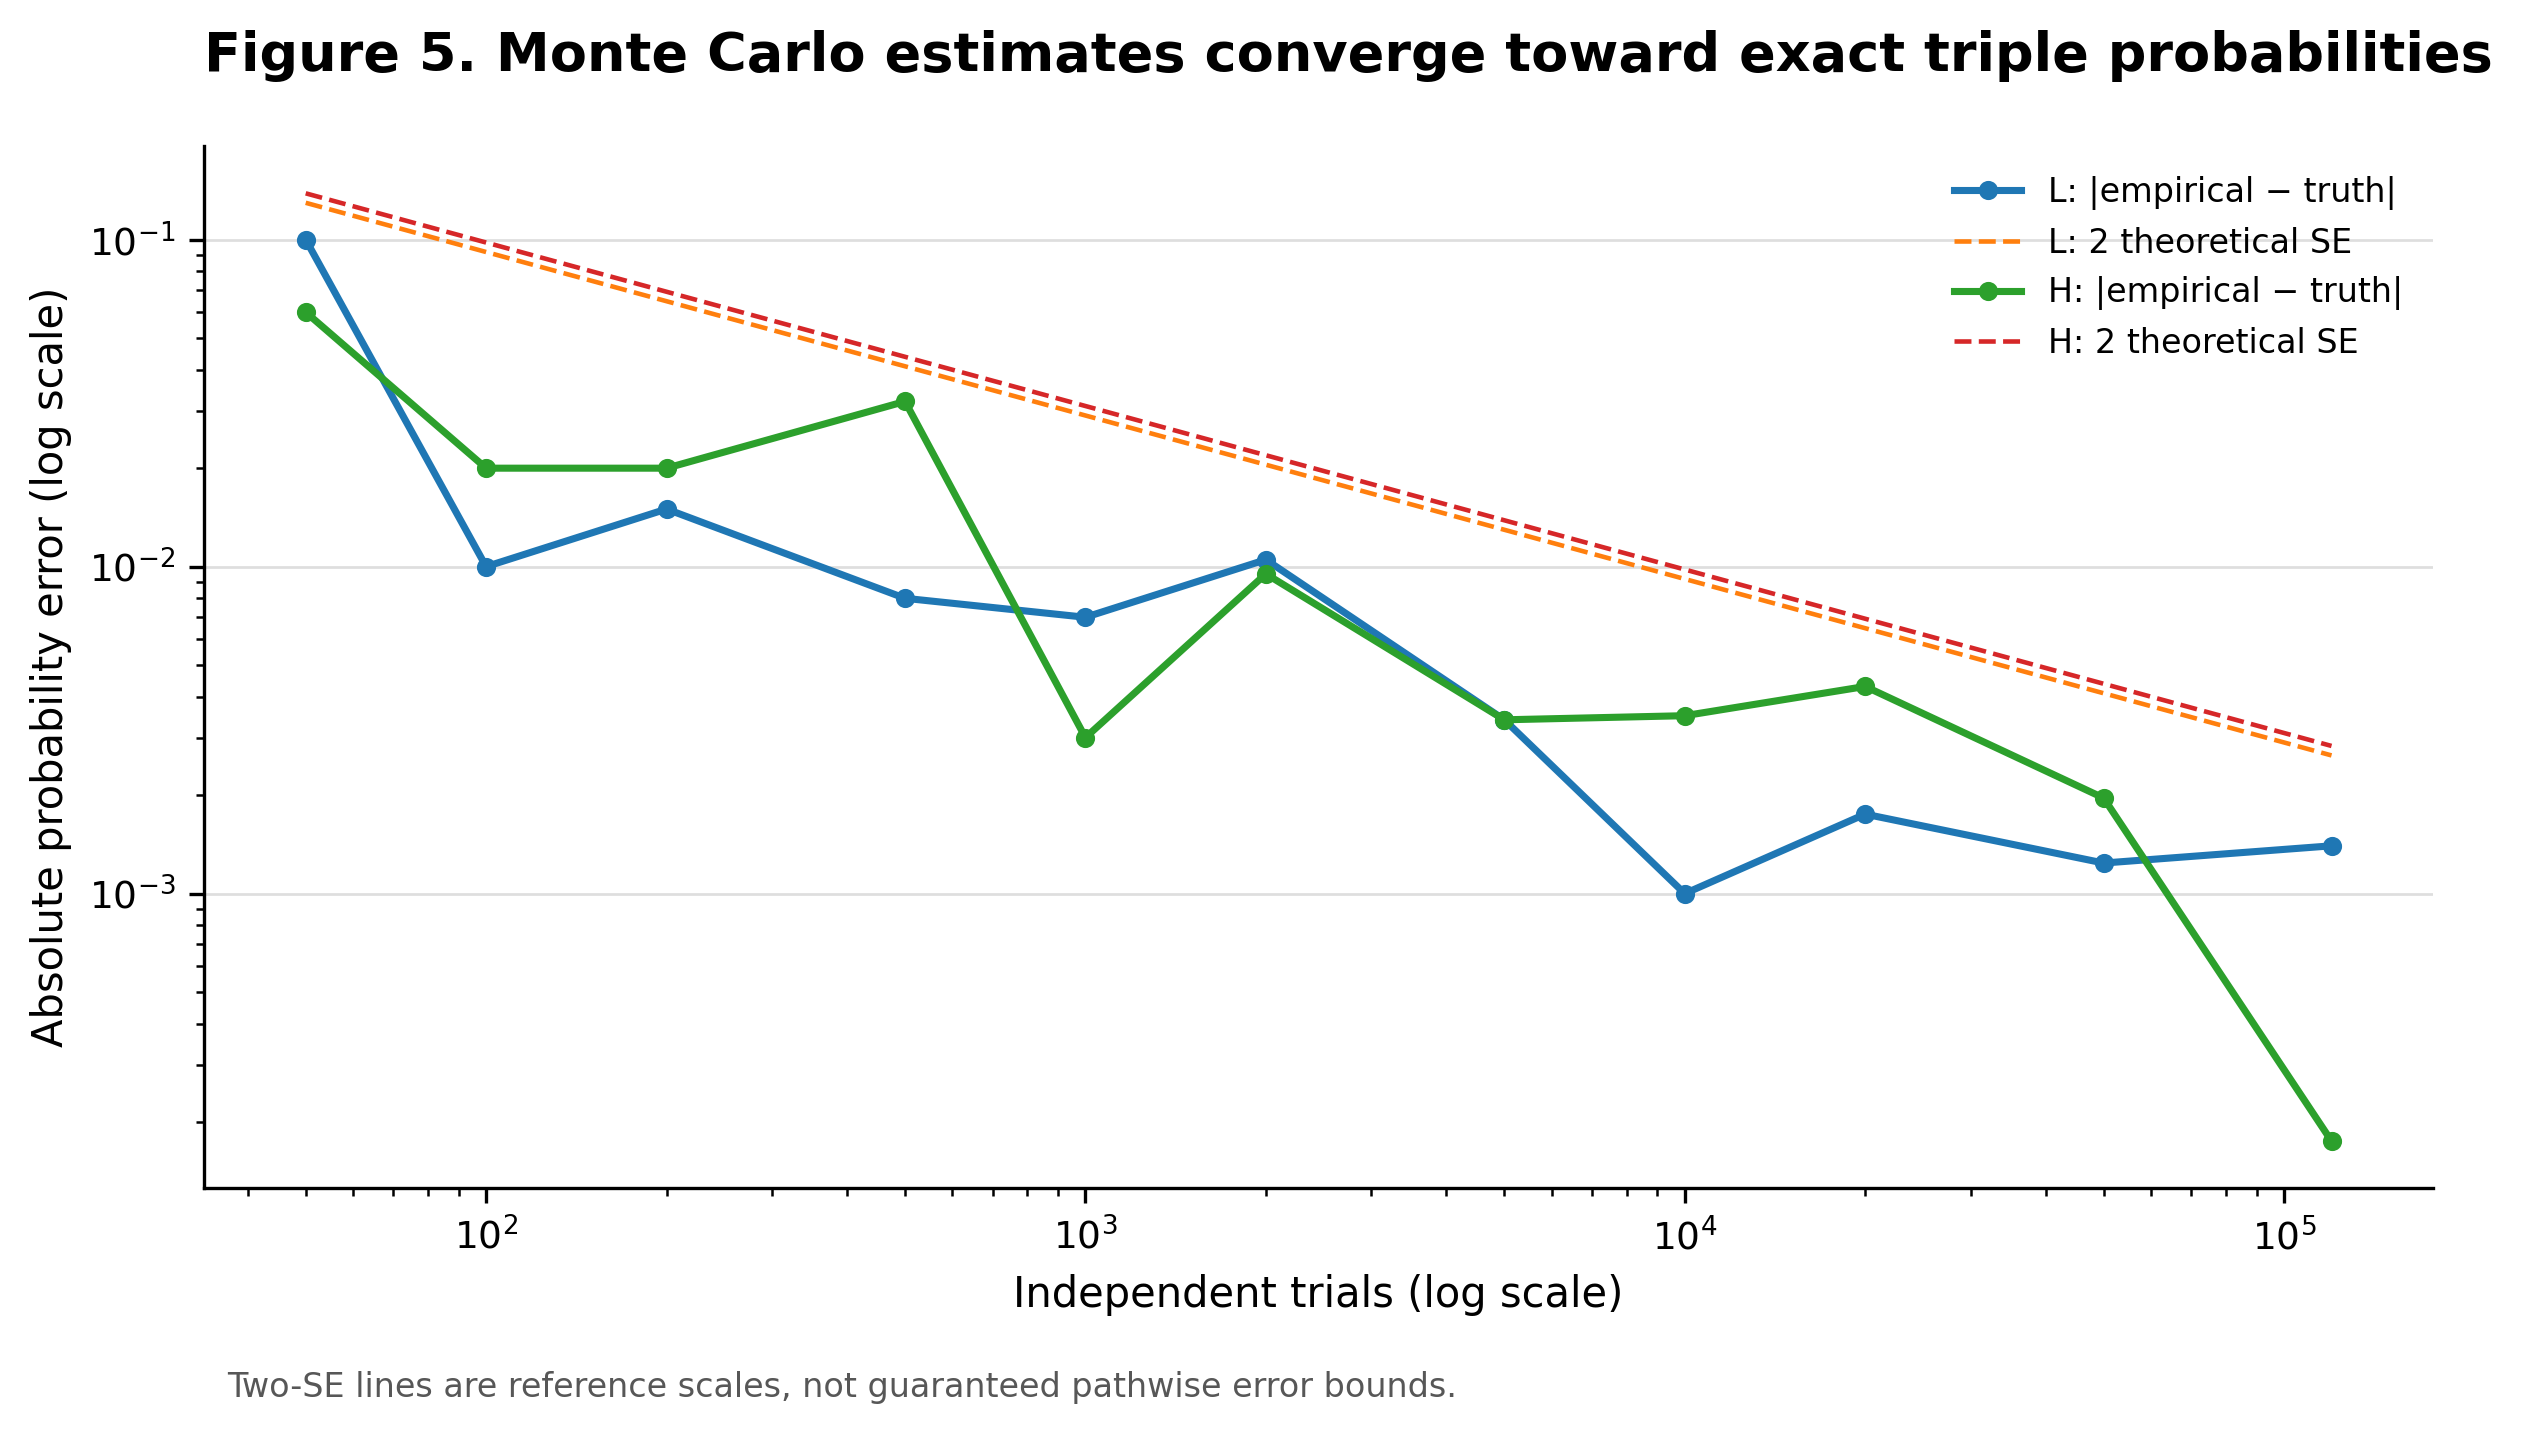
\includegraphics[width=.89\linewidth]{figures/fig05_convergence.png}
\caption{\textbf{Simulation convergence diagnostics.} Absolute estimation errors for the triple-success models compared against a reference $n^{-1/2}$ scale; sampling errors need not decrease on every increment.}\label{fig:convergence}
\end{figure}

\section{Audit, interpretation, and limitations}

\textbf{Exact verification.} A fresh Phase 6 script, distinct from the original simulation implementation, checks the source ZIP and its 43 SHA-256 manifest entries, recomputes ranking and triple-distribution identities using rational arithmetic, solves a three-coin sharp-bound linear program, verifies the finite-extension construction, and recalculates exact binomial identification probabilities and selected recorded statistics. It reports 133 passing checks. The Phase 5 audit was also replayed from a fresh extraction and passed; it includes regeneration of earlier-phase tests and figure files. These machine checks support internal consistency but are not external peer review.

\textbf{What the results establish.} Within the stated mathematical models: contradictory same-context zero-sum guarantees are impossible; fixed high marginal probabilities do not identify a joint-success probability; extending finite symmetry introduces genuine restrictions; low-order observations can conceal higher-order dependence; and a reliability-allocation ranking can depend on a fixed coupling.

\textbf{What they do not establish.} The analysis does not establish original mathematical theorems, measure Lucky Coin probabilities, authenticate specific numerical statements about any webtoon episode, identify a unique physical or fictional mechanism, or show that one illustrative resource strategy is globally best under arbitrary dependence. The source series is a creative motivation, not a probability dataset. The simulated confidence intervals describe repeated draws from stipulated distributions; they are not uncertainty intervals for any fictional world parameter.

\textbf{Research positioning.} The mathematical ingredients are established. The educational contribution is the integrated sequence of explicit paradoxes, constructed countermodels, sharp constraints, simulations, and identification limits. This manuscript should be considered for an expository venue or mathematical-essay setting; a primary research journal would require an independently validated contribution beyond these established results.

\section{Conclusion}

``Absolute luck'' is not a complete probabilistic statement. Two players may both have a 99\% chance against a baseline opponent while their mutual duel remains unidentified. Two hundred coins can each be 99.5\% reliable while collective success is impossible, unless additional structure rules out that dependence law. Observing each coin and every pair may still fail to determine what happens to the triple. A policy that best distributes a reliability boost under independence may be inferior under another fixed joint mechanism. These are not failures of the probability axioms. They are consequences of changing the event, context, observation protocol, or dependence assumptions. The resolution is mathematical specification, not supernatural arithmetic.

\appendix
\section{Finite probability feasibility as a linear program}
For $n$ Bernoulli outcomes, assign masses $x_s\ge0$ to all $s\in\{0,1\}^n$, subject to $\sum_s x_s=1$ and $\sum_{s:s_i=1}x_s=p_i$. The joint-success probability is the mass on $s=(1,\ldots,1)$. Minimizing and maximizing that mass over the feasible simplex reproduces the sharp bounds \eqref{eq:bounds}. Additional moment or observational constraints can be added linearly. This is a standard finite-dimensional formulation, not a new optimization method \cite{hoppe}.

\section{Reproducibility and preserved provenance}
The full Phase 5 ZIP, including its unchanged Phase 2--4 history, is preserved under \texttt{archive/}. Its SHA-256 checksum is
\begin{center}\ttfamily\footnotesize d43e99eebcbc0842a0df9b6e03ee717b833b816ffb5d9a5cb9c7cb7beb060a3f\end{center}
The Phase 5 manifest covers 43 archived files; all 43 checksums match. The Phase 6 audit program is \texttt{audit/phase6\_independent\_checks.py}, and the machine-readable result is \texttt{audit/phase6\_audit.json}. The preserved Phase 5 experiment source and all five plots are included in the companion package. Run the Phase 6 exact audit with Python, NumPy, and SciPy; run the archived Phase 5 reproduction with its own supplied \texttt{requirements.txt}. Software versions can affect bitwise reproducibility across machines.

\begin{thebibliography}{99}
\bibitem{webtoon} S. Kim, \emph{Hardcore Leveling Warrior}, WEBTOON, official series page, \url{https://www.webtoons.com/en/action/hardcore-leveling-warrior/list?title_no=1221}. Used as creative source identification only; specific probability mechanics not independently authenticated.
\bibitem{bradley} R. A. Bradley and M. E. Terry, ``Rank Analysis of Incomplete Block Designs: I. The Method of Paired Comparisons,'' \emph{Biometrika}, vol. 39, nos. 3--4, pp. 324--345, 1952. \url{https://doi.org/10.1093/biomet/39.3-4.324}.
\bibitem{luce} R. D. Luce, ``Luce's choice axiom,'' \emph{Scholarpedia}, vol. 3, no. 12, p. 8077, 2008. \url{https://doi.org/10.4249/scholarpedia.8077}.
\bibitem{hoppe} F. M. Hoppe and M. Nediak, ``Fr\'echet optimal bounds on the probability of a union with supplementary information,'' \emph{Statistics \& Probability Letters}, vol. 78, no. 3, pp. 311--319, 2008. \url{https://doi.org/10.1016/j.spl.2007.02.019}.
\bibitem{kirsch} W. Kirsch, ``An elementary proof of de Finetti's theorem,'' \emph{Statistics \& Probability Letters}, vol. 151, pp. 84--88, 2019. \url{https://doi.org/10.1016/j.spl.2019.03.014}.
\bibitem{konstantopoulos} T. Konstantopoulos and L. Yuan, ``On the extendibility of finitely exchangeable probability measures,'' \emph{Transactions of the American Mathematical Society}, vol. 371, no. 10, pp. 7067--7092, 2019. \url{https://doi.org/10.1090/tran/7701}.
\bibitem{shaked} M. Shaked and J. G. Shanthikumar, ``Optimal allocation of resources to nodes of parallel and series systems,'' \emph{Advances in Applied Probability}, vol. 24, no. 4, pp. 894--914, 1992. \url{https://doi.org/10.2307/1427718}.
\bibitem{brown} L. D. Brown, T. T. Cai, and A. DasGupta, ``Interval Estimation for a Binomial Proportion,'' \emph{Statistical Science}, vol. 16, no. 2, pp. 101--117, 2001; associated published discussion and rejoinder extend through p. 133. \url{https://doi.org/10.1214/ss/1009213286}.
\end{thebibliography}
\end{document}